\documentclass[conference]{IEEEtran}
\IEEEoverridecommandlockouts
% The preceding line is only needed to identify funding in the first footnote. If that is unneeded, please comment it out.
\usepackage{cite}
\usepackage{amsmath,amssymb,amsfonts}
\usepackage{graphicx}
\usepackage{textcomp}
\usepackage{xcolor}
\def\BibTeX{{\rm B\kern-.05em{\sc i\kern-.025em b}\kern-.08em
    T\kern-.1667em\lower.7ex\hbox{E}\kern-.125emX}}
\begin{document}

\title{Crime Prediction Using Hotel Customer Reviews\\
{\footnotesize https://github.com/robroooh/txt-mng}
}

\author{\IEEEauthorblockN{Somkiadcharoen Robroo}
\IEEEauthorblockA{\textit{Faculty of Information Technology} \\
\textit{and Electrical Engineering} \\
\textit{University of Oulu}\\
Oulu, Finland \\
robroo.pc@gmail.com}
\and
\IEEEauthorblockN{Bofan Lin}
\IEEEauthorblockA{\textit{Faculty of Information Technology} \\
\textit{and Electrical Engineering} \\
\textit{University of Oulu}\\
Oulu, Finland \\
bofan.lin@student.oulu.fi}
}

\maketitle

\begin{abstract}
Can hotel customer reviews be used as a proxy for predicting crime hotspots? It becomes a hot issue recently. Tourists are prime targets for criminals. Therefore, tourists and visitors should remain alert, attentive, and vigilant to suspicious activities and can be used as reliable "human crime sensors". We proposed a novelty analysis method to enhance the features from hotel reviews dataset. And compared the London crime heat map with the hotel data map. Spatial clustering and sentiment feedback The result is likely that the features that we get from both dataset are from different perspective and might not applicable to translate the knowledge to this domain.
\end{abstract}

\begin{IEEEkeywords}
Crime Prediction, Spatial Clustering, Sentiment Analysis, Heat Map, Hotel, Review,
\end{IEEEkeywords}

\section{Introduction}
Crimes are a potential problem in the world. The wellbeing and the trust of the society are affected by crimes, and there is no significant drop in the crime rate until now TODO: add a citation. One way to reduce the crime rate can be done by putting more effort into creating more advanced analytics platform to sense and predict the crime. The problem is challenging since there is no absolute way to infer it directly, even though there are many effort spending on existing dataset such as Twitter Posts \cite{autocrimepred}, Demographics and Mobile Data \cite{towardscrimepred}. Can hotel customer reviews be used as a proxy for predicting crime hotspots?
\section{Background}

\subsection{Problems}
Crimes are usually recorded according to a specific group of location, which can determined a specific group of location as a whole whether the crime has occurred or not. With the help of the hotel reviews data, heuristically, there might be some correlation with how the users feel with the crimes that are happened in the same area since the users might feel uncomfortable living around the area that are unsafe in a way.

The purpose of this work is to try to synthesize two different sets of data which are hotel review data, and crime record data. This study will help us get more understanding about the crime rate and how the customers perceive hotels. Because hotel reviews are known to be a perception of how users feel about hotel, where the feel is purely subjective and might correlate with insecure feeling they have during the stay. The combination of these 2 data would give us more information towards predicting crimes.

\subsection{Datasets}\label{AA}
Here we employed the use of 2 different dataset for different purpose. The first one is a hotel review dataset which is likely to infer to the quality of the hotel service. Another one is a crime dataset from Police.

\subsubsection{TripAdvisor hotel reviews dataset}
We used the customer reviews dataset which contains about 140,000 customer reviews from hotels in London, and includes 15 features as shown in Table \ref{tab:attributes}.

\begin{table}[h]
\centering
\caption{The attributes of two datasets.}
\label{tab:attributes}
    \begin{tabular}{r|l|l}
      \textbf{Column} & \textbf{Hotel Review Dataset} & \textbf{Metropolitan Crime Dataset}\\
      \hline
      1 & Hotel Name & Crime ID\\
      2 & Hotel Review Stars & Month\\
      3 & Hotel Address & Reported by\\
      4 & City & Falls within\\
      5 & ZIP & Longitude\\
      6 & Review Title & Latitude\\
      7 & Review Date & Location\\
      8 & Review Content & LSOA code\\
      9 & Review Stars & LSOA name\\
      10 & Reviewer Name & Crime type\\
      11 & Reviewer Location & Last outcome category\\
      12 & Reviewer Profile & Context\\
      13 & Reviewer Total Reviews&\\
      14 & Reviewer Hotel Reviews &\\
      15 & Helpful Votes &\\
    \end{tabular}
\end{table}

\subsubsection{Crime Heatmaps Visualization}
Visualize crimes happened in London on a heat map.

\subsubsection{England Police Metropolitan Crime Dataset}
downloaded from https://data.police.uk/
The data is selected from 3/2017 - 8/2017
The metropolitan-street.csv dataset includes 12 features as shown in Table \ref{tab:attributes}.

\section{Methods}
We hypothesized that hotels with more negative ratings would be the ones that are in high crime rate, and the positive rating hotels would yield opposite result, as compared with each group. To test this hypothesis, we extracted a textual feature, use them to enhance the existing features, and combined those 2 data and spatially analyse the correlation between the data.

\subsubsection{Geo-coding Conversion}
The hotel reviews datasets only contains the hotel address, in order the harmonize those two datasets, we have to convert the address to latitude and longitude. It is also helpful for the further analysis.

\subsubsection{Features Extraction}
In order to analysis the hidden information of the hotel reviews, we have to use sentiment analysis method to extract at least three new features. For example, how was the service the hotel and how was the environment around the hotel.

\subsubsection{Hotel Features Visualization}
In order to explore the spatial dimensions of the data, we can visualize the structured data on the map. With the help of some machine learning methods, to define our observations are independent or identically distributed.

\subsection{Geo-coding Conversion}
In order to harmonize the existing 2 datasets, the preprocessing on the address of these must be done. The hotel reviews data only have the address as a text, while the crime data provide both text and spatial location. It is done using the Google's Geocoding API to decode the hotel address to the Latitude and Longitude. In the original data, there are some missing values of Hotel Address. For those hotels, we convert the Hotel Name and City to Latitude and Longitude.

\subsection{Features Extraction}
The deep learning based sentiment analysis in this project is based on hotel review titles. The library in used is the StanfordCoreNLP [TODO: add githublink]. It is a NLP toolkit from stanford which provides many aspects of the texts to be used. However, we are only interested in the sentimental analysis of the reviewer. The sentiment is done only to the review titles since we tried them on both review titles and review texts, but the results are not significantly better and took longer time to inference. Also, heuristically we can infer the sentiment of the review by just reading the heading of the review. The pre-processing task is done by using a Python wrapper of StanfordCoreNLP[TODO: add github link] to detect the level of sentiment where the possibilities are Verynegative, Negative, Neutral, Postive, Verypositive. With the help of luck, these results can be directly map to the review star ratings column with the value of 1-5 where the sentiment will be used to find the Effective Rating Score and perform a Fraud detection. There are 3 features that are extracted from the hotel reviews dataset as the followings

\subsubsection{EFF (Effective Rating Score)}
The intuition behind the EFF based on the biases of the reviewers. This can be illustrated in the following case. Given that there are two reviewers gave the same review score of 3, but one of them said "Quite Bad Hotel" and another one said "OK". We can see in this example that the meaning of 3 varies on perspectives of the people. Therefore, we would like to use the sentiment and the review ratings to compute whether they go together in the same way. The processing in this step can be seen in 2 cases.  The first case is same direction. It means that if the review score is good (4-5) and the sentiment is also good (Positive, Verypositive), the rating score is valid. The same goes for the negative direction. If the score comes out quite bad (1-2) and the sentiment goes to the same direction of (Negative, Verynegative), the rating score is valid and should be kept, also done the same with Neutral rating and score of 3. The second one is the contradict. If the rating score is good, but the sentiment goes bad, the rating of this one is not invalid, and it won't be used to calculate anything further than this. The same goes with the rating score of 3 and sentiment other than Neutral.

\subsubsection{DIST (Distance from a crime spot)}
The intuition behind this is that the hotel that are close to crime spots are supposed to have a worse review. In the column of in the hotel data and column in the crime data, we foresee that there is a table which has the name occurred on TODO which can be used to use the direct text map, where the result is that 90\% of them can be mapped directly. After the map, we use a Python package called hola to compute the (harvestine) distance between two spatial location.

\subsubsection{AVG\_CRIME\_N (Average occurrence of crime per month)}
The intuition of this is just to inference another features on the average crime that is occurred between 6 months timeframe. it can be easily seen as number of crime over number of month.

\subsection{Visualization}
\subsubsection{Hotel Features Visualization}
We downloaded an 'England.json' file from the internet. And we used those three features that we extracted before, to cluster the hotels into three classes by Kmeans which provided by sklearn package.Then we plot the result by maplotlib. As shows in the Figure \ref{fig:hotelsmap}.

\begin{figure}[h]
  \centering
  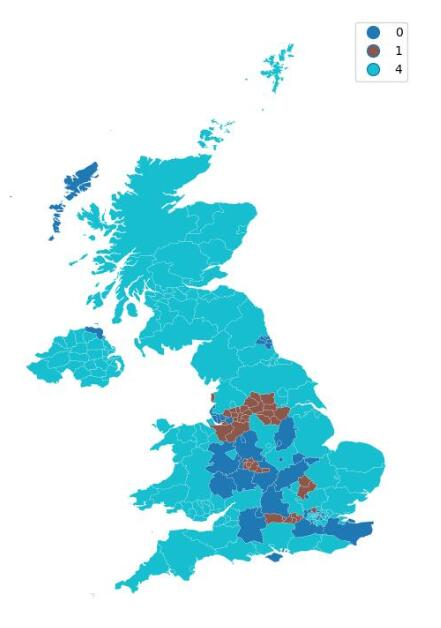
\includegraphics[width=4cm,height=6cm]{Hotels.jpg}
  \caption{Hotels}
  \label{fig:hotelsmap}
\end{figure}

\subsubsection{Crime Heatmaps Visualization}
We used the England Police Metropolitan Crime Dataset which contains the data from 3/2017 to 8/2017. The result shows that the crime is almost everywhere in London. As shows in the  Figure \ref{fig:crimemap}.

\begin{figure}[h]
  \centering
  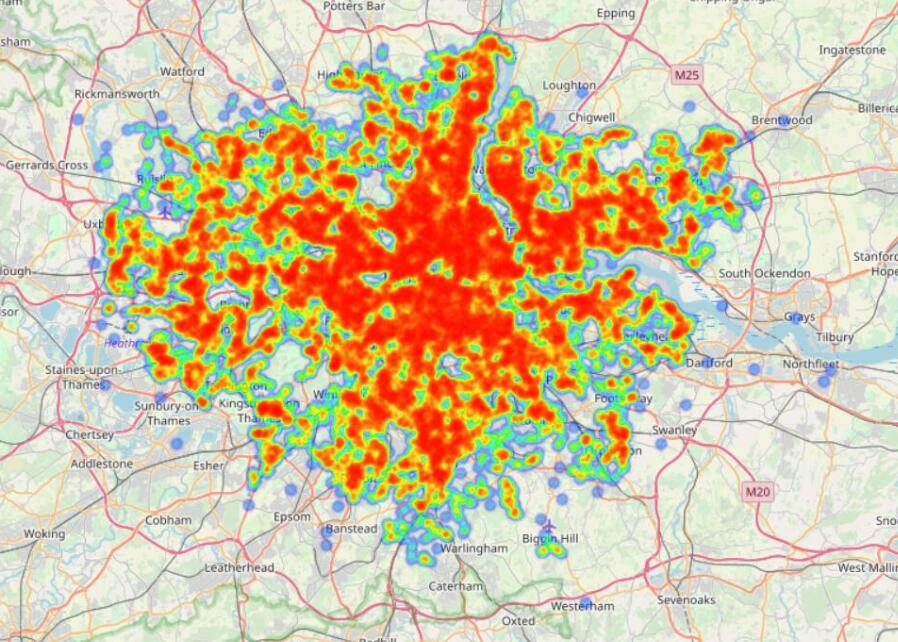
\includegraphics[width=9cm,height=5cm]{Heatmap.jpg}
  \caption{Crime Heatmap}
  \label{fig:crimemap}
\end{figure}

\subsection{Data Analysis}
\subsubsection{Fraud Detection}
\subsubsection{Correlation and Causalities Analysis}
\subsubsection{Spatial Correlation}
\section{Results \& Discussion}
We initially think that the hotel reviews should directly related to the fact that how the service of specific hotels are perceived by customers, and thus would not have any direct correlation or causalities on the crime dataset. After the ad-hoc analysis before the visualization phase, the data seems to us that it might not work well in this case, and we do not have enough backup plan to put any additional dataset into solving this problem. In addition, the experiences of us related to text mining in this case is quite basic, given that we only did the sentiment analysis on the hotel review and use those results to enhance the existing knowledges that we have. We feel like we could have done it better if we have more experience in this.
\section{Conclusion}
We presented the methodology to detect crime using hotel reviews. The results are based on those 2 datasets only which are TripAdvisor hotel review dataset and England's Metropolitan police crime dataset.
\section{Future Work}
We learned that this project is a pure combination between art and science. As both of us do not have prior knowledge in dealing with text data and spatial data before, we were a bit lost in the first place. However, with the rise of popularity in the NLP field, it helps us to be able to find the references to guide us on what we should work on, and that was only the guideline. This kind of work is likely to make use of both creativity and technical skills to solve.

We would love to know more on how to heuristically solve this project. Moreover, it would be great to ask for opinions from people in the industry who are working on this to roughly know how they tackle this kind of project. We suggested to develop this work further by combining more modalities of the data in addition to dig deeper on textual features which might not help getting a significantly better result due to the nature of the dataset.

\appendix[Source Code \& Datasets]
The Python source codes are publicly available on the GitHub link https://github.com/robroooh/txt-mng. It


\begin{thebibliography}{00}
\bibitem{autocrimepred} Wang X., Gerber M.S., Brown D.E. (2012) Automatic Crime Prediction Using Events Extracted from Twitter Posts. In: Yang S.J., Greenberg A.M., Endsley M. (eds) Social Computing, Behavioral - Cultural Modeling and Prediction. SBP 2012. Lecture Notes in Computer Science, vol 7227. Springer, Berlin, Heidelberg.
\bibitem{towardscrimepred} Andrey Bogomolov , Bruno Lepri , Jacopo Staiano , Nuria Oliver , Fabio Pianesi , Alex Pentland, Once Upon a Crime: Towards Crime Prediction from Demographics and Mobile Data, Proceedings of the 16th International Conference on Multimodal Interaction, November 12-16, 2014, Istanbul, Turkey.
\bibitem{b3} I. S. Jacobs and C. P. Bean, ``Fine particles, thin films and exchange anisotropy,'' in Magnetism, vol. III, G. T. Rado and H. Suhl, Eds. New York: Academic, 1963, pp. 271--350.
\bibitem{b4} K. Elissa, ``Title of paper if known,'' unpublished.
\bibitem{b5} R. Nicole, ``Title of paper with only first word capitalized,'' J. Name Stand. Abbrev., in press.
\bibitem{b6} Y. Yorozu, M. Hirano, K. Oka, and Y. Tagawa, ``Electron spectroscopy studies on magneto-optical media and plastic substrate interface,'' IEEE Transl. J. Magn. Japan, vol. 2, pp. 740--741, August 1987 [Digests 9th Annual Conf. Magnetics Japan, p. 301, 1982].
\bibitem{b7} M. Young, The Technical Writer's Handbook. Mill Valley, CA: University Science, 1989.
\end{thebibliography}
\end{document}
